The United States have been the forerunner of nuclear energy, with a current
installed capacity of about 100 GWe. With its size and long history of nuclear
energy, the United States have accumulated about $70,000$ \gls{MTHM} of \gls{UNF}.
The United States' historical nuclear operation and inventory is tracked using
\Cyclus and is compared with benchmarked results from \gls{ORION} and the
\gls{UNF-STANDARDS} database. The \gls{UNF-STANDARDS} database is a comprehensive,
controlled source of \gls{UNF} information, including dry cask attributes, assembly
data, and economic attributes \cite{peterson_unf-st&dards_2017}. With the successful benchmark,
the simulation is extrapolated to the future. I run two separate simulations, 
one with transition into a `closed' fuel cycle, and the other once-through.

The problem with modeling the U.S. transition scenario is that the U.S. does not have
a defined advanced reactor, whereas France has a central plan to transition into \glspl{ASTRID} \cite{boullis_french_2015, varaine_pre-conceptual_2012}.
Although the most prominent and `canonical' reactor design when considering
transition is the \gls{SFR}, the fact that the U.S. nuclear reactor fleet
is decided by economic interests (industries), this allows me to explore
different options, such as the \gls{MSR} design.

\iffalse
To appropriately model the U.S. \gls{UNF} inventory, I imported the
\gls{UNF-STANDARDS} database to accurately model the U.S. \gls{UNF}
inventory in 2013. Starting from 2013, I run a similar simulation to
that of France. Since the U.S. did not reprocess its \gls{UNF}, it
has a significant amount of plutonium obtainable from its current
inventory. However, the current \gls{DOE} policy is to not reprocess
fuel discharged prior to 2013, since it expects that the U.S. will
accumulate enough \gls{LWR} \gls{UNF} by the time \gls{FR} reactors
are ready for commercial deployment \cite{worrall_utilization_2013}.
However, this study assumes the \gls{FR} available year to be
2050, with a nuclear energy demand growth rate of 1\% per year.
\fi

I investigate the effects of availability year and nuclear energy
demand growth rate in the waste metrics, and whether the U.S. will
need to reprocess its pre-2013 \gls{UNF} to transition.

Also, I compare the results of transitioning into a \gls{SFR} fleet
and into a \gls{MSR} fleet, and how transitioning into two different designs
affect the final material inventory.

\section{Methodology}

Since the U.S. has a significant amount of \gls{LWR} \gls{UNF}
to separate plutonium from, I chose a \gls{SFR} design that has a low breeding ratio.
Previous studies \cite{worrall_utilization_2013} show that plutonium inventory
is not a limiting factor to the success of transition. Thus, the purpose
of the U.S. transition case is guided towards minimizing the waste inventory
and utilizing the currently available resources (\gls{LWR} \gls{UNF} and
depleted uranium).

\subsection{Predicting the Past - Pre-2013 inventory}
The pre-2013 \gls{UNF} inventory is modeled using the \gls{UNF-STANDARDS}
database. The database provides the fuel composition of all assemblies
discharged before 2013. I imported the fuel composition of the assemblies
after one year of decay and used Python Nuclear Engineering Toolkit (PyNE) \cite{scopatz_pyne_2012}
to decay the assemblies to 2013, to obtain the effective fuel mass and composition
in 2013.

\subsection{Predicting the Future}
I used a similar approach to model the current and future nuclear fleet of the
U.S. as I did for France. I used the \gls{IAEA} \gls{PRIS} database to populate
the \Cyclus input file to model the current U.S. fleet. Reactors that do not
have a defined decommission date are assumed to have a lifetime to 60 years.

To meet the increasing power demand, I deploy \glspl{PWR} (AP1000 design)
until the \gls{FR} available date. After the \gls{FR} available date,
I deploy \glspl{FR} to meet the increasing power demand.

\subsection{Reactor Specification}
Three major reactors are used in this study, \gls{PWR}, \gls{SFR}, and
\gls{MSR} reactors.

I modeled the \gls{PWR} after the AP-1000 reactor design \cite{sutharshan_ap1000tm_2011},
the \gls{SFR} after the \gls{ABR} design \cite{kim_core_2009}, and the 
\gls{MSR} after the \gls{UK} \gls{MCSFR} design \cite{smith_assessment_1974}. The \gls{ABR} has two regions -
a fissile driver and a blanket region. The two regions are modeled separately in \Cyclus,
to account for the different cycle times, mass and composition. Table \ref{tab:reactor} shows
the reactor specifications. 


\begin{table}[h]
    \centering
    \caption{Baseline \gls{LWR} and \gls{ASTRID} simulation specifications.}
    \begin{tabular}{lrrrr}
        \hline
        \textbf{Specification} & \textbf{\gls{PWR} \cite{sutharshan_ap1000tm_2011}} & \textbf{\gls{ABR} - Driver \cite{kim_core_2009}} & \textbf{\gls{ABR} - Blanket \cite{kim_core_2009}} & \textbf{\gls{MCSFR} \cite{smith_assessment_1974}}\\
        \hline
                Lifetime [y]  & 80 & 80 & 80 & 20 \\
                Cycle Time [mos.]& 18 & 9 & 14 & -\\ 
                Refueling Outage [mos.]& 1 & 1 & 1 & -\\
                Rated Power [\gls{MWe}] & 1000 & 400 & 0 & 820\\
                Batch mass [kg] & 29,565 & 3,076 & 768 & 43,300\\
                Batches per core & 3 & 5 & 5 & 1\\
                Discharge Burnup [GWd/tHM] & 51 & 67 & - & - \\
                Initial Fissile Loading [t] & 2.74  $^{235}$U & 2.30 $Pu$ & 2.59 $Pu$ \\
                Fuel & UOX & U-Pu-Zr Metal & U-Zr Metal & U-Pu-Na-Cl \\
        \hline
    \end{tabular}
        
    \label{tab:reactor}

    \end{table}

The \gls{MCSFR} behaves differently than the \gls{PWR} and the \gls{SFR}, in
that it discharges material and refuels continuously. Thus, its material flow
and parameters are not defined by discrete batch sizes, but rates of discharge
and fertile material intake. The \gls{MCSFR} parameters used for the simulation
are listed in table \ref{tab:msr}.

\begin{table}[h]
    \centering
    \caption{\gls{MCSFR} Parameters}
    \begin{tabular}{ll}
        \hline
        Parameter & Value \\
        \hline
        Fertile intake material & Depleted uranium \\
        Fertile intake rate & 1,190 kg /year\\ 
        Fissile output material & plutonium \\
        Fissile output rate & 330 kg /year \\
        Waste output material & Fission products \\
        Waste output rate & 870 kg /year \\
        \hline
    \end{tabular}
    \label{tab:msr}
\end{table}


\subsection{Material Definitions}
Depletion calculations of the nuclear fuel are recipe-based, such that a 
fresh and used fuel recipe is defined for each reactor type. For the compositions
of the used fuel, a reference depleteion calculation from ORIGEN is used (see
table \ref{tab:comp}). ORIGEN calculates buildup, decay, and processing of 
radioactive materials \cite{parks_overview_1992}. The recipe is generated as
part of the FCDP database project %%%%CITE%%%%%%.

\begin{table}[h]
    \centering
    \caption{Fresh fuel compositions in the simulation} %CITEEEE
%   \scalebox{0.86}{
        \begin{tabular}{lrrr}
            \hline
             & \multicolumn{3}{c}{ Composition [\%]} \\
            Recipe & U-235  & U-238  & Pu \\ 
            \hline
            Fresh \gls{UOX} Fuel & 3.1 & 96.9 & -   \\ 
            Fresh \gls{SFR} Driver & 0.34 & 84.66 & 15 \\ 
            Fresh \gls{SFR} Blanket & 0.7 & 99.3 & 0 \\
            Fresh \gls{MSR} Fuel Salt & 0.28 & 93.72 & 6 \\
            \hline
        \end{tabular}
        \label{tab:sim_result}
\end {table}


\subsection{Parameter sweep of transition scenarios to \gls{SFR} fleet}
I performed a parameter sweep of transition scenarios to
a \gls{SFR} fleet starting from 2013. The parameters used in the
sweep are listed in table \ref{tab:params}.

\begin{table}[h]
    \centering
    \begin{tabular}{cc}
        \hline
        Parameters & Values \\
        \hline
        Energy Demand Growth Rate [\% per year] & 0, 0.5, 1, 1.5 \\
        \gls{SFR} available year & 2030, 2035, 2040, 2045, 2050\\
        Pre-2013 \gls{UNF} inventory & Yes, No \\
        \hline
    \end{tabular}
    \caption{Parameter ranges for transition scenario}
    \label{tab:params}
\end{table}


\subsection{Difference in Reactor Design - \gls{MSR} vs \gls{SFR}}
As mentioned above, the U.S. does not have a central advanced
reactor design it is pursuing, like France. There has been
a recent upsurge of interest in \gls{MSR} designs, that are
reflected by numerous nuclear start-ups such as Terrapower,
Terrestrial Energy, ThorCon Power, and Transatomic Power
Corporation. \gls{MSR} designs are unique in the way
that the material flow in and out of the reactor is
continuous and not discrete, like \glspl{LWR} and \glspl{SFR}.
Also, the liquid-fuel nature of an \gls{MSR} design allows
for on-line reprocessing, which reduces the initial fissile
loading due to elimination of the need for excess reactivity in the core at startup.
Since poisons are removed during operation of a \gls{MSR}, it has 
better neutron economy, thus better resource utilization.

I compare the transition scenario of the U.S. nuclear fleet with
transition starting from 2050 and with an energy demand increase
rate of 1.5\%, to observe difference in metrics with the difference
in deployed reactor design.


\section{Results}




\subsection{Parameter sweep of transition scenarios to \gls{SFR} fleet}

The parameters sweep of transition scenarios to \gls{SFR} fleet provides
insight into the effects of parameters changes to the metric values. 

Failed transition scenarios are listed in table \ref{tab:trans_fail}. Failure
of transition means that a deployed \gls{SFR} was not able to produce power
due to lack of fuel. The lack of fuel is caused by a lack of plutonium inventory, which
means that the transition year was too soon (without enough \gls{LWR} \gls{UNF}) or
that the \gls{SFR} deployment was too steep, due to the annual energy demand growth.
As shown in table \ref{tab:trans_fail}, most scenarios successfully transitions into
a fully-\gls{SFR} fleet, even without the pre-2013 \gls{LWR} \gls{UNF} inventory.
With the pre-2013 \gls{LWR} \gls{UNF} inventory, three more transition scenarios
succeed. 


\begin{figure}
\begin{tabular}{cc|cccc}
   \hline
   & & \multicolumn{4}{c}{Annual Energy Demand Growth Rate [\%]} \\
   & & 0 & 0.5 & 1.0 & 1.5 \\
    \hline
   &2030 &
  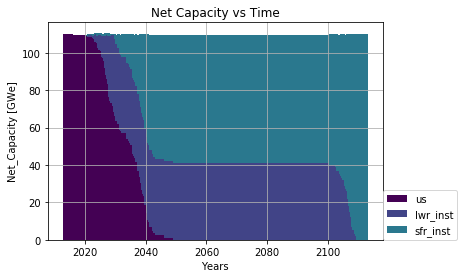
\includegraphics[width=0.2\textwidth]{./us/powers/2030_0_growth_precise.png} &
  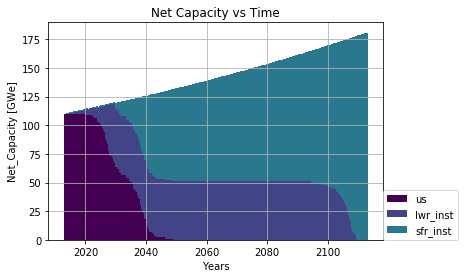
\includegraphics[width=0.2\textwidth]{./us/powers/2030_005_growth_precise.png} &
  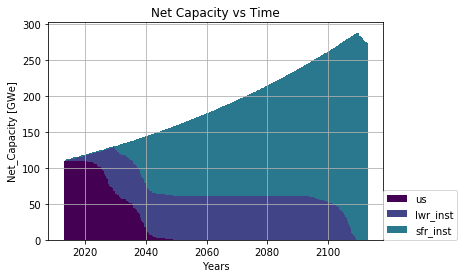
\includegraphics[width=0.2\textwidth]{./us/powers/2030_01_growth_precise.png} &
  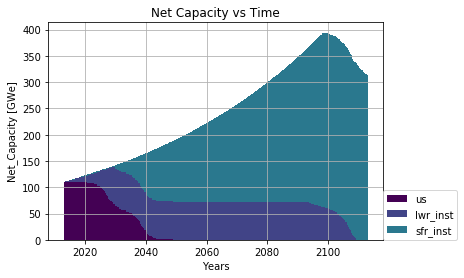
\includegraphics[width=0.2\textwidth]{./us/powers/2030_015_growth_precise.png} \\
  
  \multirow{4}{*}{\shortstack{\\ \\ \gls{SFR} \\ \\ \\ Available \\ \\ \\ Year}}&2035 &
  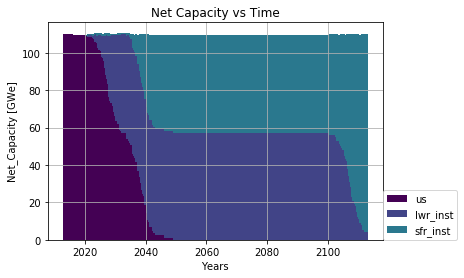
\includegraphics[width=0.2\textwidth]{./us/powers/2035_0_growth_precise.png} &
  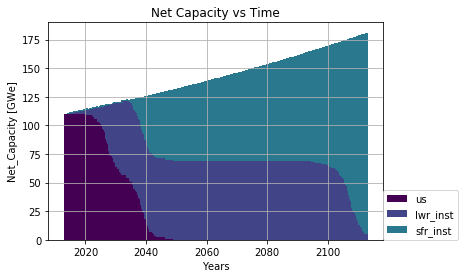
\includegraphics[width=0.2\textwidth]{./us/powers/2035_005_growth_precise.png} &
  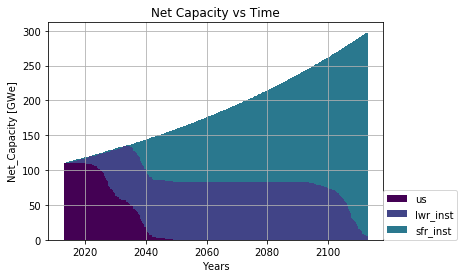
\includegraphics[width=0.2\textwidth]{./us/powers/2035_01_growth_precise.png} &
  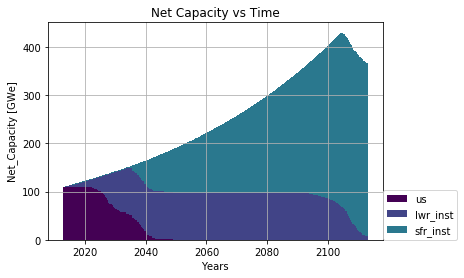
\includegraphics[width=0.2\textwidth]{./us/powers/2035_015_growth_precise.png} \\
  
  &2040 &
  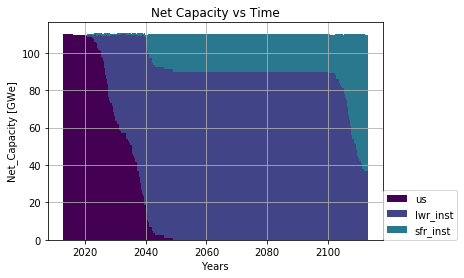
\includegraphics[width=0.2\textwidth]{./us/powers/2040_0_growth_precise.png} &
  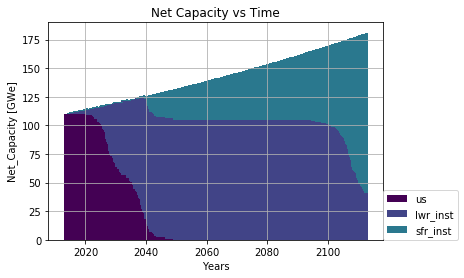
\includegraphics[width=0.2\textwidth]{./us/powers/2040_005_growth_precise.png} &
  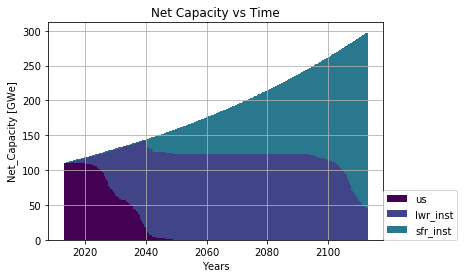
\includegraphics[width=0.2\textwidth]{./us/powers/2040_01_growth_precise.png} &
  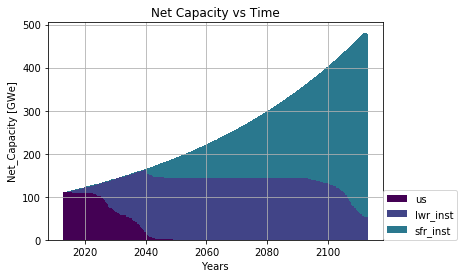
\includegraphics[width=0.2\textwidth]{./us/powers/2040_015_growth_precise.png} \\
  
  &2045 &
  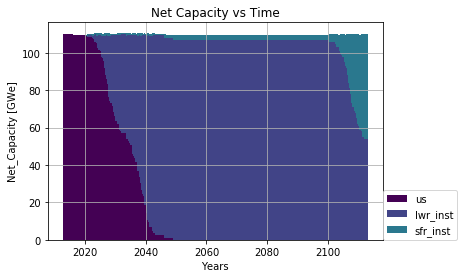
\includegraphics[width=0.2\textwidth]{./us/powers/2045_0_growth_precise.png} &
  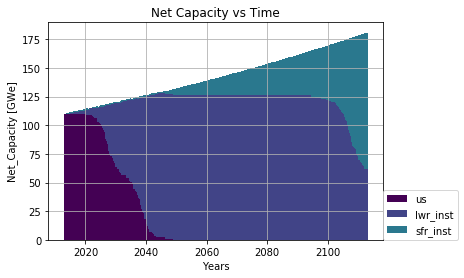
\includegraphics[width=0.2\textwidth]{./us/powers/2045_005_growth_precise.png} &
  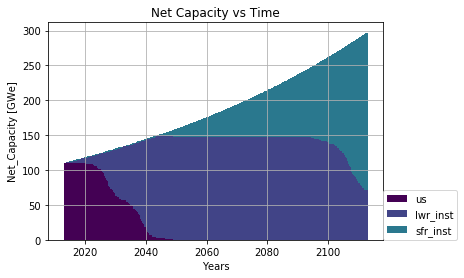
\includegraphics[width=0.2\textwidth]{./us/powers/2045_01_growth_precise.png} &
  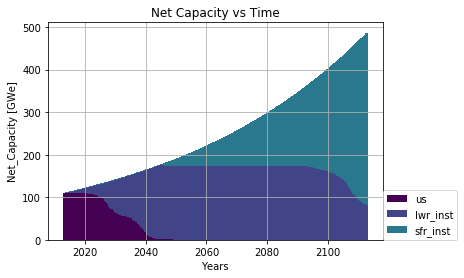
\includegraphics[width=0.2\textwidth]{./us/powers/2045_015_growth_precise.png} \\
  
  &2050 &
  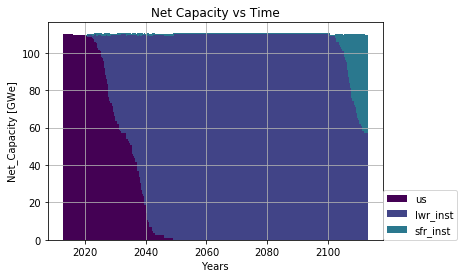
\includegraphics[width=0.2\textwidth]{./us/powers/2050_0_growth_precise.png} &
  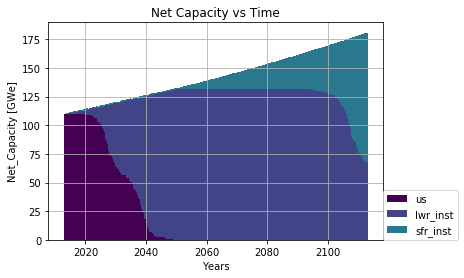
\includegraphics[width=0.2\textwidth]{./us/powers/2050_005_growth_precise.png} &
  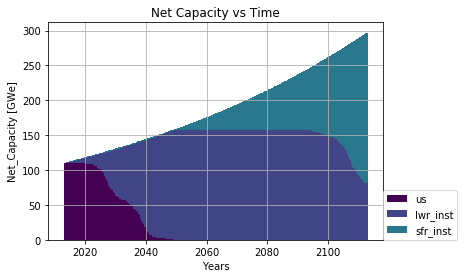
\includegraphics[width=0.2\textwidth]{./us/powers/2050_01_growth_precise.png} &
  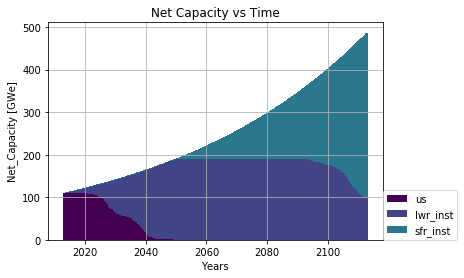
\includegraphics[width=0.2\textwidth]{./us/powers/2050_015_growth_precise.png} \\
  
\end{tabular}
\caption{Installed power capacity changes for all scenarios in the parameter sweep study.}
\end{figure}

\begin{table}[h]
    \centering
    \begin{tabular}{cc|cccc}
    \hline
    & & \multicolumn{4}{c}{Energy Demand Growth Rate [\%]} \\
    & & 0 & 0.5 & 1.0 & 1.5 \\
    \hline
    & 2030 & - & \textcolor{blue}{WOL}& \textcolor{red}{ALL} & \textcolor{red}{ALL} \\
    \multirow{4}{*}{\shortstack{\gls{SFR} \\ \\ Available \\ \\ Year}}& 2035 & - & - & \textcolor{blue}{WOL} & \textcolor{red}{ALL} \\
    & 2040 & - & - & - & \textcolor{blue}{WOL} \\
    & 2045 & - & - & - & - \\
    & 2050 & - & - & - & - \\
    \hline
    \end{tabular}
    \caption{Transition failure cases. `\textcolor{blue}{WOL}' denotes failure only when legacy \gls{UNF} is not reprocessed. `\textcolor{red}{ALL}' denotes transition failure even with reprocessing legacy \gls{UNF}.}
    \label{tab:trans_fail}
\end{table}


\begin{figure}%
    \centering
    \subfloat{{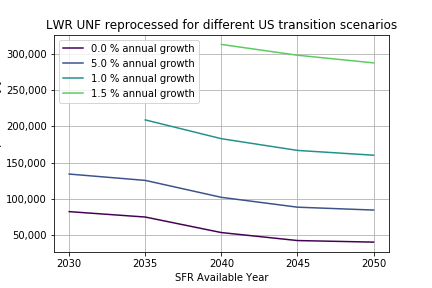
\includegraphics[width=0.45\textwidth]{./images/us/y_LWR_UNF_reprocessed.png} }}%
    \qquad
    \subfloat{{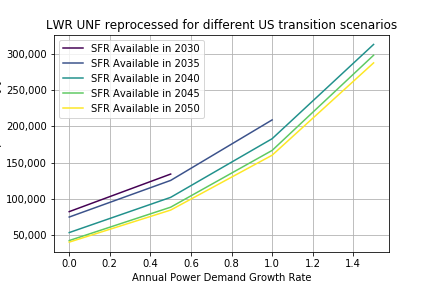
\includegraphics[width=0.45\textwidth]{./images/us/g_LWR_UNF_reprocessed.png} }}%
    \caption{\gls{LWR} \gls{UNF} Reprocessed for each simulation}%
    \label{fig:us_lwr_unf_rep}%
\end{figure}

\begin{figure}%
    \centering
    \subfloat{{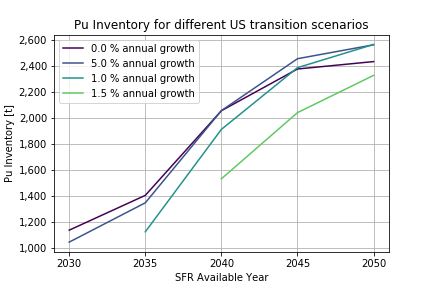
\includegraphics[width=0.45\textwidth]{./images/us/y_Pu_Inventory.png} }}%
    \qquad
    \subfloat{{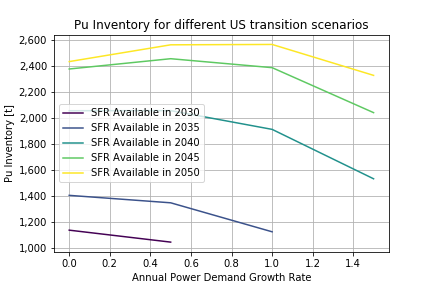
\includegraphics[width=0.45\textwidth]{./images/us/g_Pu_Inventory.png} }}%
    \caption{Outstanding plutonium inventory for each simulation}%
    \label{fig:us_pu_inv}%
\end{figure}

\begin{figure}%
    \centering
    \subfloat{{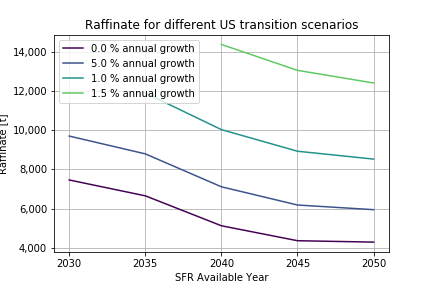
\includegraphics[width=0.45\textwidth]{./images/us/y_Raffinate.png} }}%
    \qquad
    \subfloat{{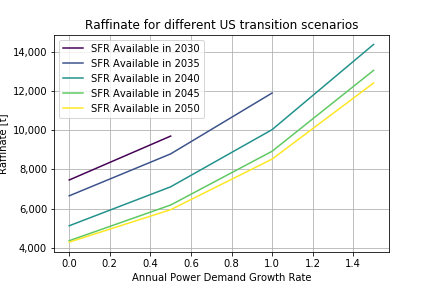
\includegraphics[width=0.45\textwidth]{./images/us/g_Raffinate.png} }}%
    \caption{Raffinate inventory for each simulation}%
    \label{fig:us_raff}%
\end{figure}

\begin{figure}%
    \centering
    \subfloat{{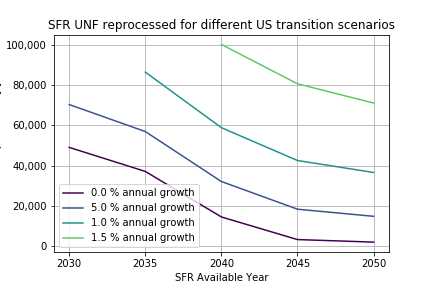
\includegraphics[width=0.45\textwidth]{./images/us/y_SFR_UNF_reprocessed.png} }}%
    \qquad
    \subfloat{{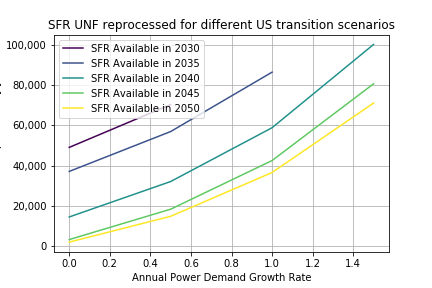
\includegraphics[width=0.45\textwidth]{./images/us/g_SFR_UNF_reprocessed.png} }}%
    \caption{\gls{SFR} \gls{UNF} Reprocessed for each simulation}%
    \label{fig:sfr_unf_rep}%
\end{figure}

\begin{figure}%
    \centering
    \subfloat{{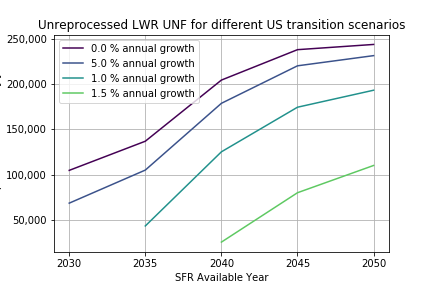
\includegraphics[width=0.45\textwidth]{./images/us/y_Unreprocessed_LWR_UNF.png} }}%
    \qquad
    \subfloat{{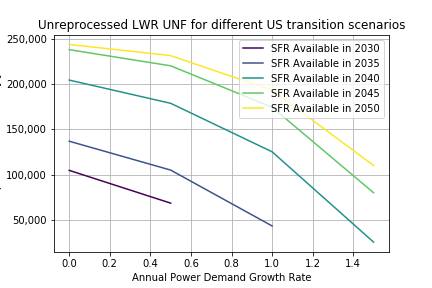
\includegraphics[width=0.45\textwidth]{./images/us/g_Unreprocessed_LWR_UNF.png} }}%
    \caption{Oustanding \gls{LWR} \gls{UNF} inventory for each simulation}%
    \label{fig:lwr_unf_reproc}%
\end{figure}



%%%% SCAT BOTH
The metric values and their sensitivity to the parameters are shown in figures
\ref{fig:us_lwr_unf_rep, fig:us_raff, fig:us_pu_inv, fig:us_sfr_unf_rep, fig:us_lwr_unf_rep}.
The colors show the magnitude of the metric, where a darker color means that the metric has a
lower numerical value. The arrows in between the two regions symbolize the direction and magnitude
of the increase in metric with their neighboring points (i.e. $\frac{dz}{dx}$, $\frac{dz}{dy}$). For example, a large arrow facing right
means that the metric value largely increases when there is an increase in annual power
demand growth rate.

Figure \ref{fig:us_lwr_unf_rep} shows that the mass of \gls{LWR} \gls{UNF} has a large
range within the parameters, from $50,000$ to $300,000$ tons. 
The amount of \gls{LWR} \gls{UNF} increases with increase
in power demand growth rate, and decreases with the delay in
\gls{SFR} available year. The decrease is primariliy due to
the late introduction of the \glspl{SFR} in the simulation. The annual power demand
growth rate has a large influence (average increase of $55,780 \text{MTHM} (58.4 \%)$ 
per 0.5 percent increase) to the amount of \gls{LWR} \gls{UNF}
reprocessed. On the other hand, the change in  \gls{SFR} available year
has less of an effect (average decrease of $9,757 \text{MTHM} (8.22\%)$
per 5 year delay).


\begin{figure}[htbp!]
    \begin{center}
        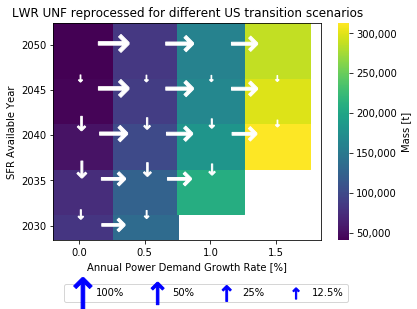
\includegraphics[scale=0.7]{./images/us/scat_both_LWR_UNF_reprocessed.png}
    \end{center}
        \caption{\gls{LWR} \gls{UNF} Reprocessed for each simulation}
    \label{fig:us_lwr_unf_rep}
\end{figure}


Figure \ref{fig:us_lwr_unf_rep} shows that the mass of \gls{SFR} \gls{UNF} reprocessed.
The amount of \gls{SFR} \gls{UNF} reprocessed increases greatly with increase
in power demand growth rate, and decreases with the delay in
\gls{SFR} available year. The decrease is primariliy due to
the late introduction of the \glspl{SFR} in the simulation, which decreases the number of \glspl{SFR} deployed in the simulation. The annual power demand
growth rate has a large influence (average increase of $17,887 \text{MTHM} (124.38 \%)$ 
per 0.5 percent increase) to the amount of \gls{SFR} \gls{UNF}
reprocessed. On the other hand, the change in  \gls{SFR} available year
has less of an effect (average decrease of $10,723 \text{MTHM} (25.7\%)$
per 5 year delay). Note that the magnitude of percentage increase
with increase in growth rate decreases ($\frac{d^2z}{dx^2} < 0$)
because reprocessing only the \gls{SFR} \gls{UNF} cannot provide
the plutonium for \gls{SFR} fuel. Thus, \gls{LWR} \gls{UNF} is
reprocessed to compliment the plutonium demand in the higher
growth rate cases.

\begin{figure}[htbp!]
    \begin{center}
        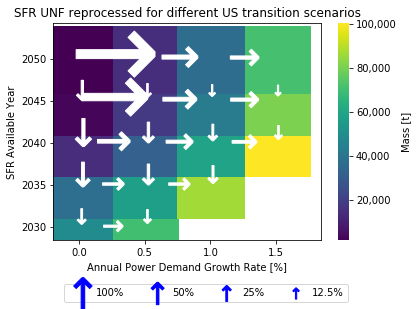
\includegraphics[scale=0.7]{./images/us/scat_both_SFR_UNF_reprocessed.png}
    \end{center}
        \caption{\gls{SFR} \gls{UNF} Reprocessed for each simulation}
    \label{fig:us_sfr_unf_rep}
\end{figure}



Figure \ref{fig:us_raff} shows that the mass of accumulated
raffinate inventory in each simulation. 
The amount of accumulated raffinate behaves similar to the
amount of \gls{LWR} \gls{UNF} reprocessed, since most 
raffinate comes from reprocessing \gls{LWR} \gls{UNF}. However, the correlation is weakened by the raffinate stream from reprocessing \gls{SFR} \gls{UNF}. The annual power demand
growth rate has a larger influence (average increase of $1,973 \text{MTHM} (22.26 \%)$ 
per 0.5 percent increase) to the amount of raffinate accumulated. On the other hand, the change in  \gls{SFR} available year
has less of an effect (average decrease of $721 \text{MTHM} (8.29\%)$
per 5 year delay).


\begin{figure}[htbp!]
    \begin{center}
        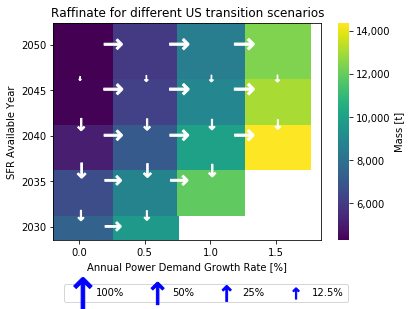
\includegraphics[scale=0.7]{./images/us/scat_both_Raffinate.png}
    \end{center}
        \caption{Raffinate Inventory for each simulation}
    \label{fig:us_raff}
\end{figure}

Figure \ref{fig:us_pu_inv} shows that the mass of accumulated
plutonium inventory in each simulation. 
The amount of plutonium inventory generally decreases with increase
in power demand growth rate, and increases with the delay in
\gls{SFR} available year. This is due to the \gls{SFR} being a
break-even core, whereas the \gls{LWR} creates extra plutonium
that is not used. Thus, having an \gls{LWR} fleet for a longer
time increases the amount of plutonium accumulated, and having
more \glspl{SFR} earlier reduces the amount of plutonium. 
Note that, unlike the other metrics, the maximum occurs in
the top center, not in the corner. This is because increased growth rate
also causes large plutonium consumption in the \glspl{SFR}. The annual power demand
growth rate has a smaller influence (average decrease of $78.7 \text{MTHM} (4.32 \%)$ 
per 0.5 percent increase) to the amount of plutonium
reprocessed. On the other hand, the change in  \gls{SFR} available year
has a bigger an effect (average increase of $297.21 \text{MTHM} (20.19\%)$
per 5 year delay).


\begin{figure}[htbp!]
    \begin{center}
        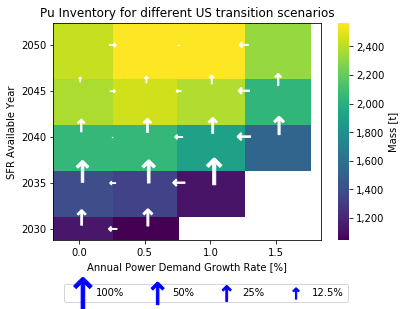
\includegraphics[scale=0.7]{./images/us/scat_both_Pu_Inventory.png}
    \end{center}
        \caption{Outstanding plutonium inventory for each simulation}
    \label{fig:us_pu_inv}
\end{figure}

Figure \ref{fig:us_lwr_unf_rep} shows that the mass of unreprocessed \gls{LWR} \gls{UNF} for each simulation. 
The amount of unreprocessed \gls{LWR} \gls{UNF} inventory decreases with increase
in power demand growth rate, and increases with the delay in
\gls{SFR} available year. This is due to the low number of 
\glspl{SFR} deployed compared to the high number of \glspl{LWR} deployed to meet the increasing power demand.  The annual power demand
growth rate has a smaller influence (average decrease of $35,269 \text{MTHM} (22.64 \%)$ 
per 0.5 percent increase) to the amount of plutonium
reprocessed. On the other hand, the change in  \gls{SFR} available year
has a bigger an effect (average increase of $31,517 \text{MTHM} (43.36\%)$
per 5 year delay). 

Note that the magnitude of the percent changes with the change
in parameters change in both directions because the metric is
affected by both the amount of \gls{SFR} fuel needed and the 
\gls{LWR} \gls{UNF} produced. These two factors are not regular
for these scenarios because \gls{SFR} deployment depends not only
on the energy demand growth rate but also on the shutdown of
\glspl{LWR}.

\begin{figure}[htbp!]
    \begin{center}
        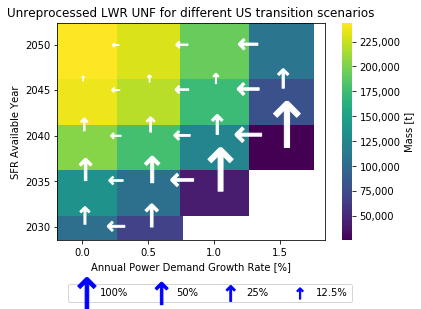
\includegraphics[scale=0.7]{./images/us/scat_both_Unreprocessed_LWR_UNF.png}
    \end{center}
        \caption{Unreproccessed \gls{LWR} \gls{UNF} for each simulation}
    \label{fig:us_lwr_unf_rep}
\end{figure}

